%%%%%%%%%%%%%%%%%%%%%%%%%%%%%%%%%%%%%%%%%%%%%%%%%%
%
%  New template code for TAMU Theses and Dissertations starting Fall 2012.  
%  For more info about this template or the 
%  TAMU LaTeX User's Group, see http://www.howdy.me/.
%
%  Author: Wendy Lynn Turner 
%	 Version 1.0 
%  Last updated 8/5/2012
%
%%%%%%%%%%%%%%%%%%%%%%%%%%%%%%%%%%%%%%%%%%%%%%%%%%%
%%%%%%%%%%%%%%%%%%%%%%%%%%%%%%%%%%%%%%%%%%%%%%%%%%%%%%%%%%%%%%%%%%%%%%
%%                           SECTION IV
%%%%%%%%%%%%%%%%%%%%%%%%%%%%%%%%%%%%%%%%%%%%%%%%%%%%%%%%%%%%%%%%%%%%%

\chapter{\uppercase{Implementation}}

The system developed in this thesis  is a TensorFlow re-implementation of  YOLO which is a fast and accurate real time object detection system originally designed by [Redmon et al., 2012]. In our implementation, we perform predictions by leveraging weights that have been trained for a long time on GPUs using ImageNet data, which is a public dataset containing millions of natural images. In our implementation, we trained the model using TensorFlow to export the graph or trained model generated using a tool called protocol buffer that  allows for easily taking advantage of the model classes in other platforms and programming languages such as mobile platforms like iOS using swift or android using java. Furthermore, we want to be able to perform real-time object tracking in live video feeds from onboard cameras on UAVs.

\section{Hardware}
We use an Nvidia GTX 1060 in our setup to benefit from faster training times in deep learning frameworks. Particularly,  TensorFlow which supports CUDA and cuDNN making neural network training significantly faster. 16GB memory to afford adding more layers to our neural network model if  required. A 256 GB SSD is used for quick access to applications and disk space for small data such as documents. A 1TB HDD is used for larger data such as stored, trained network parameters, and datasets, which quickly sum up due to copies and modifications. The CPU used is an Intel Quad-Core i7 6700HQ @ 2.6Ghz.

\pagebreak
\section{YOLO (You Only Look Once)}

YOLO is a convolutional neural network that can predict multiple-box positions and categories at once, enabling end-to-end target detection and recognition. The biggest of YOLO advantage is speed. In fact, the nature of the target detection is regression, so a CNN that implements the regression function does not require a complex design process.

YOLO avoids computationally expensive region proposal steps that detectors like Fast R-CNN[4] and Faster-RCNN[14] require. The advantage of doing so is to better distinguish between the target and the background area, compared to the use of proposal training Fast-R-CNN often the background area for a specific target. Of course, YOLO in the detection speed at the same time sacrifice some of the accuracy. 

\begin{figure}[h]
\centering
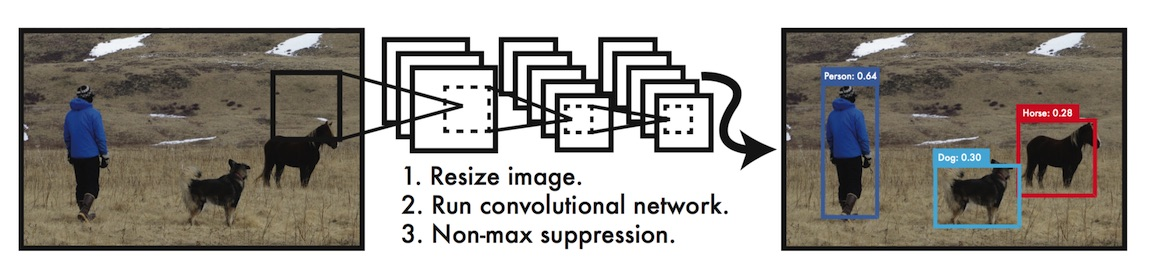
\includegraphics[scale=0.35]{figures/yolo_working.jpg}
\caption{YOLO detection system process}
\label{yolo_working}
\end{figure}

Figure \ref{yolo_working} shows the overall structure of the network :

\begin{enumerate}
\setlength{\itemsep}{-10pt}
\item Resize the image to 448 x 448.
\item Run a single convolution network.
\item Get the location and category of the object.
\end{enumerate}

\section{YOLO Network Design}

YOLO uses unified detection which unites the separate components of object detection into a single neural network. This network uses features from the entire image to predict each bounding box. This design differentiates YOLO from other methods and enables end-to-end training with real-time speeds while maintaining high average precision.  Unified detection system uses S x S grid cells and predicts B bounding boxes for each cells. Each bounding boxes produces 5 predictions: \textbf{ x},\textbf{ y}, \textbf{w}, \textbf{ h}, and confidence. The \textbf{(x,y)} is the coordinates of the center of box relative to the bounds of the grid cell. \textbf{(w,h)} is the width and height of the bounding box. The confidence score is calculated by the probability of the object multiplied by the intersection of the union of ground truth and prediction labels. Then each grid cell produce the conditional class probabilities. These probabilities are used at test time to produce the final predictions.

The final class-specific confidence scores are calculated by multiplying the conditional class probabilities with the individual box confidence predictions. The neural network architectural design includes two main components: feature extraction and prediction. The feature extraction consists of 24 convolutional layers to obtain the final 7 x 7 x 1024 activation map. This image information is passed to prediction section that has 2 fully connected layers. The probability and coordinates are produced by the last FC layer in the 7 x 7 x 30 tensor of predictions.\\

\newpage
The architecture diagram is shown in figure \ref{yolo_model} and figure \ref{yolo_net}. 

\begin{figure}[h]
\setlength{\belowcaptionskip}{-30pt}
\centering
%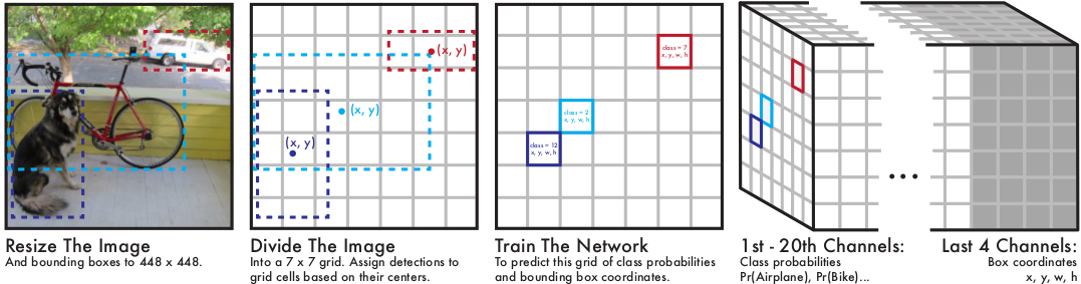
\includegraphics[scale=0.4]{figures/yolo_model.png}
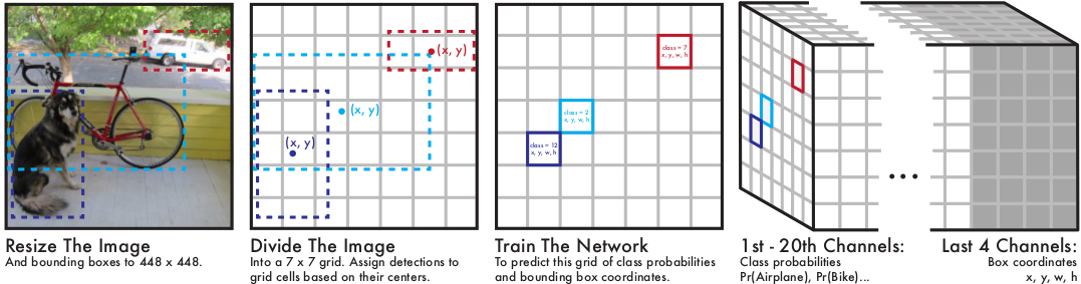
\includegraphics[width=10cm,height=12cm,keepaspectratio]{figures/yolo_model.png}
\caption{YOLO neural network prediction process}
\label{yolo_model}
\end{figure}

\begin{figure}[h]
\setlength{\belowcaptionskip}{-30pt}
\centering
%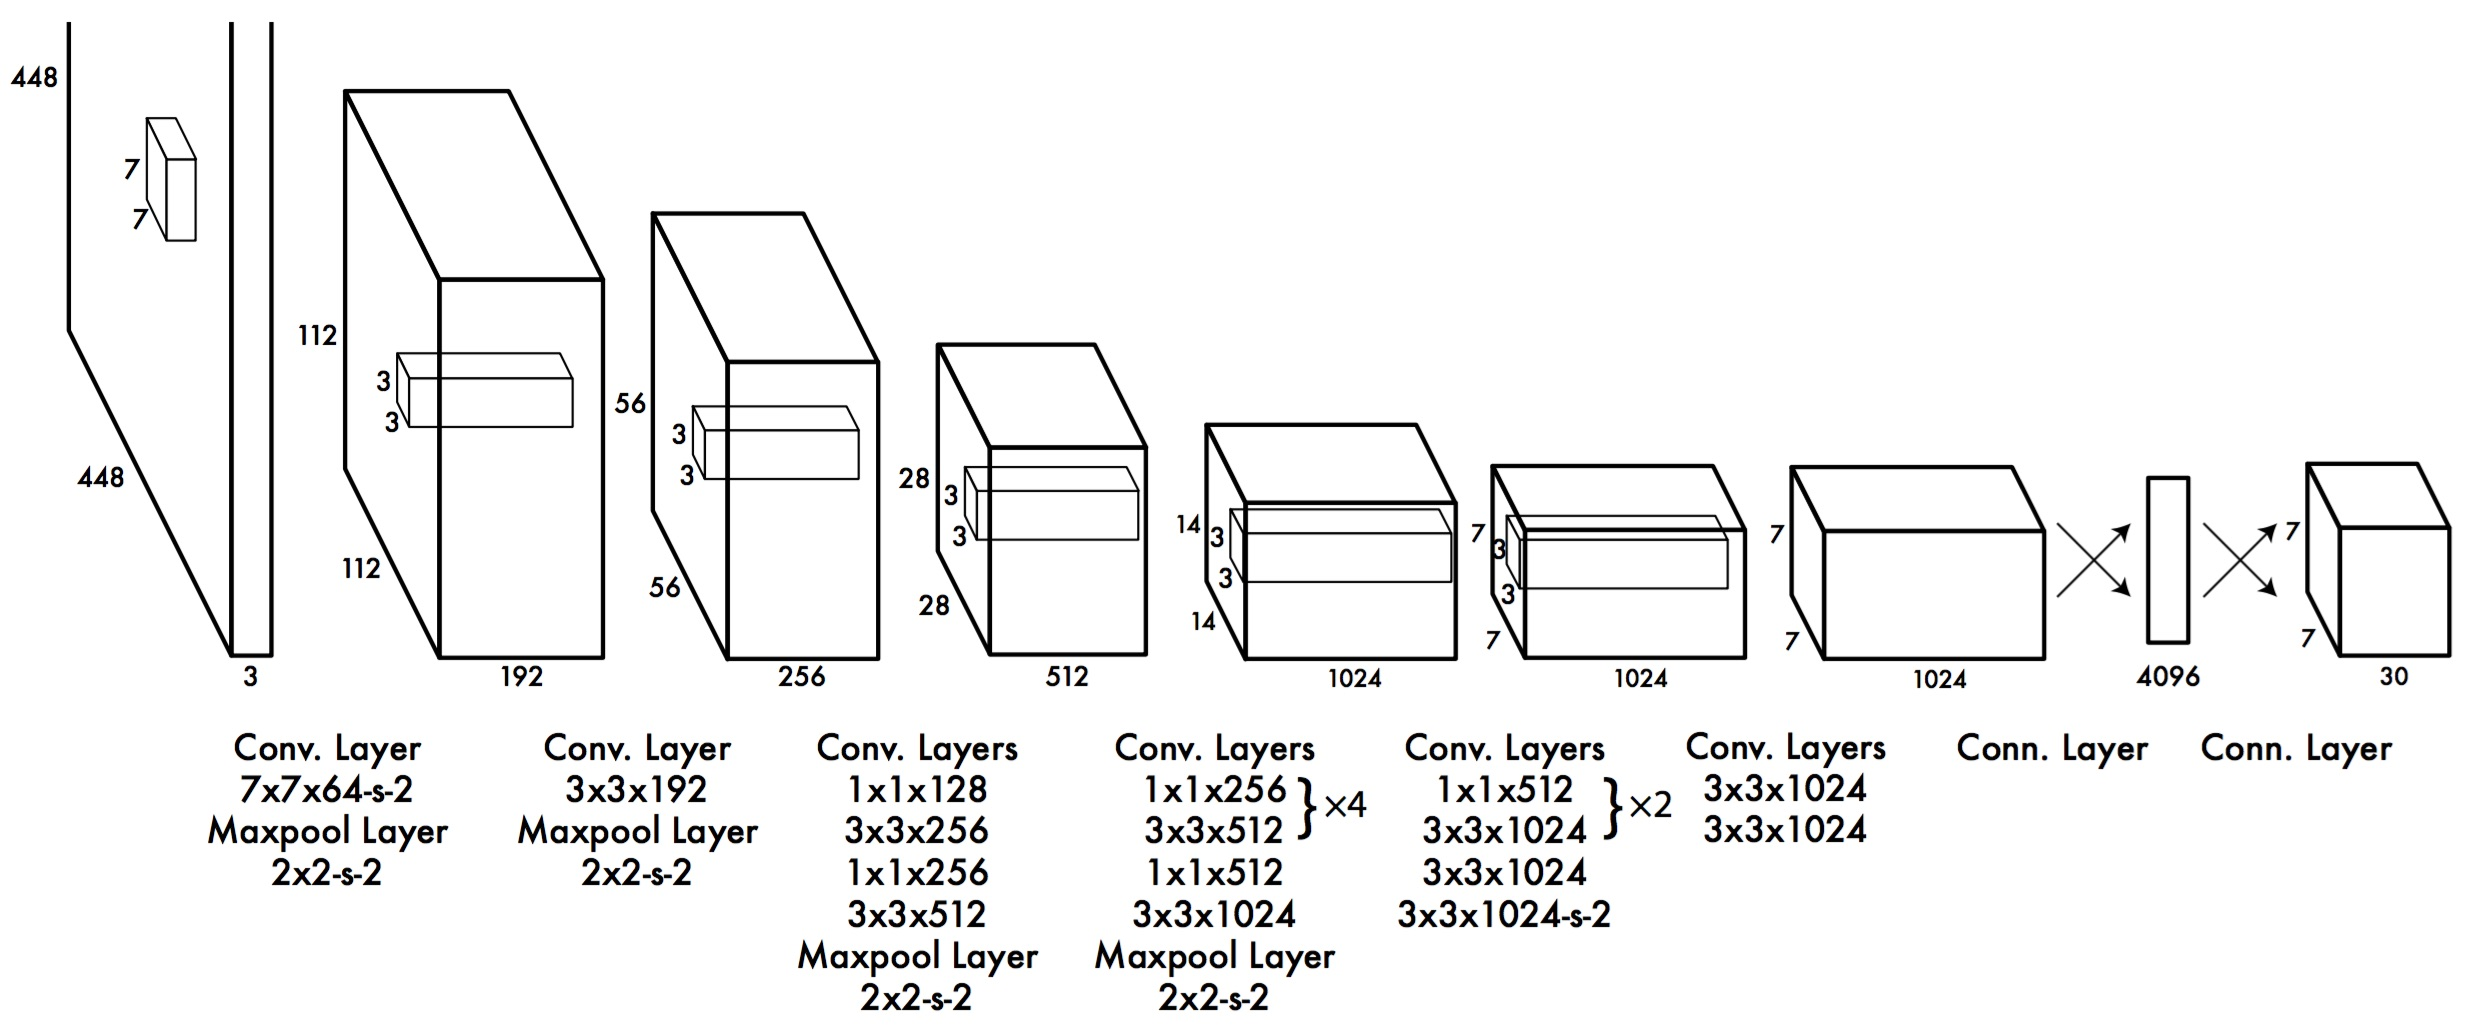
\includegraphics[scale=0.2]{figures/yolo_net.jpg}
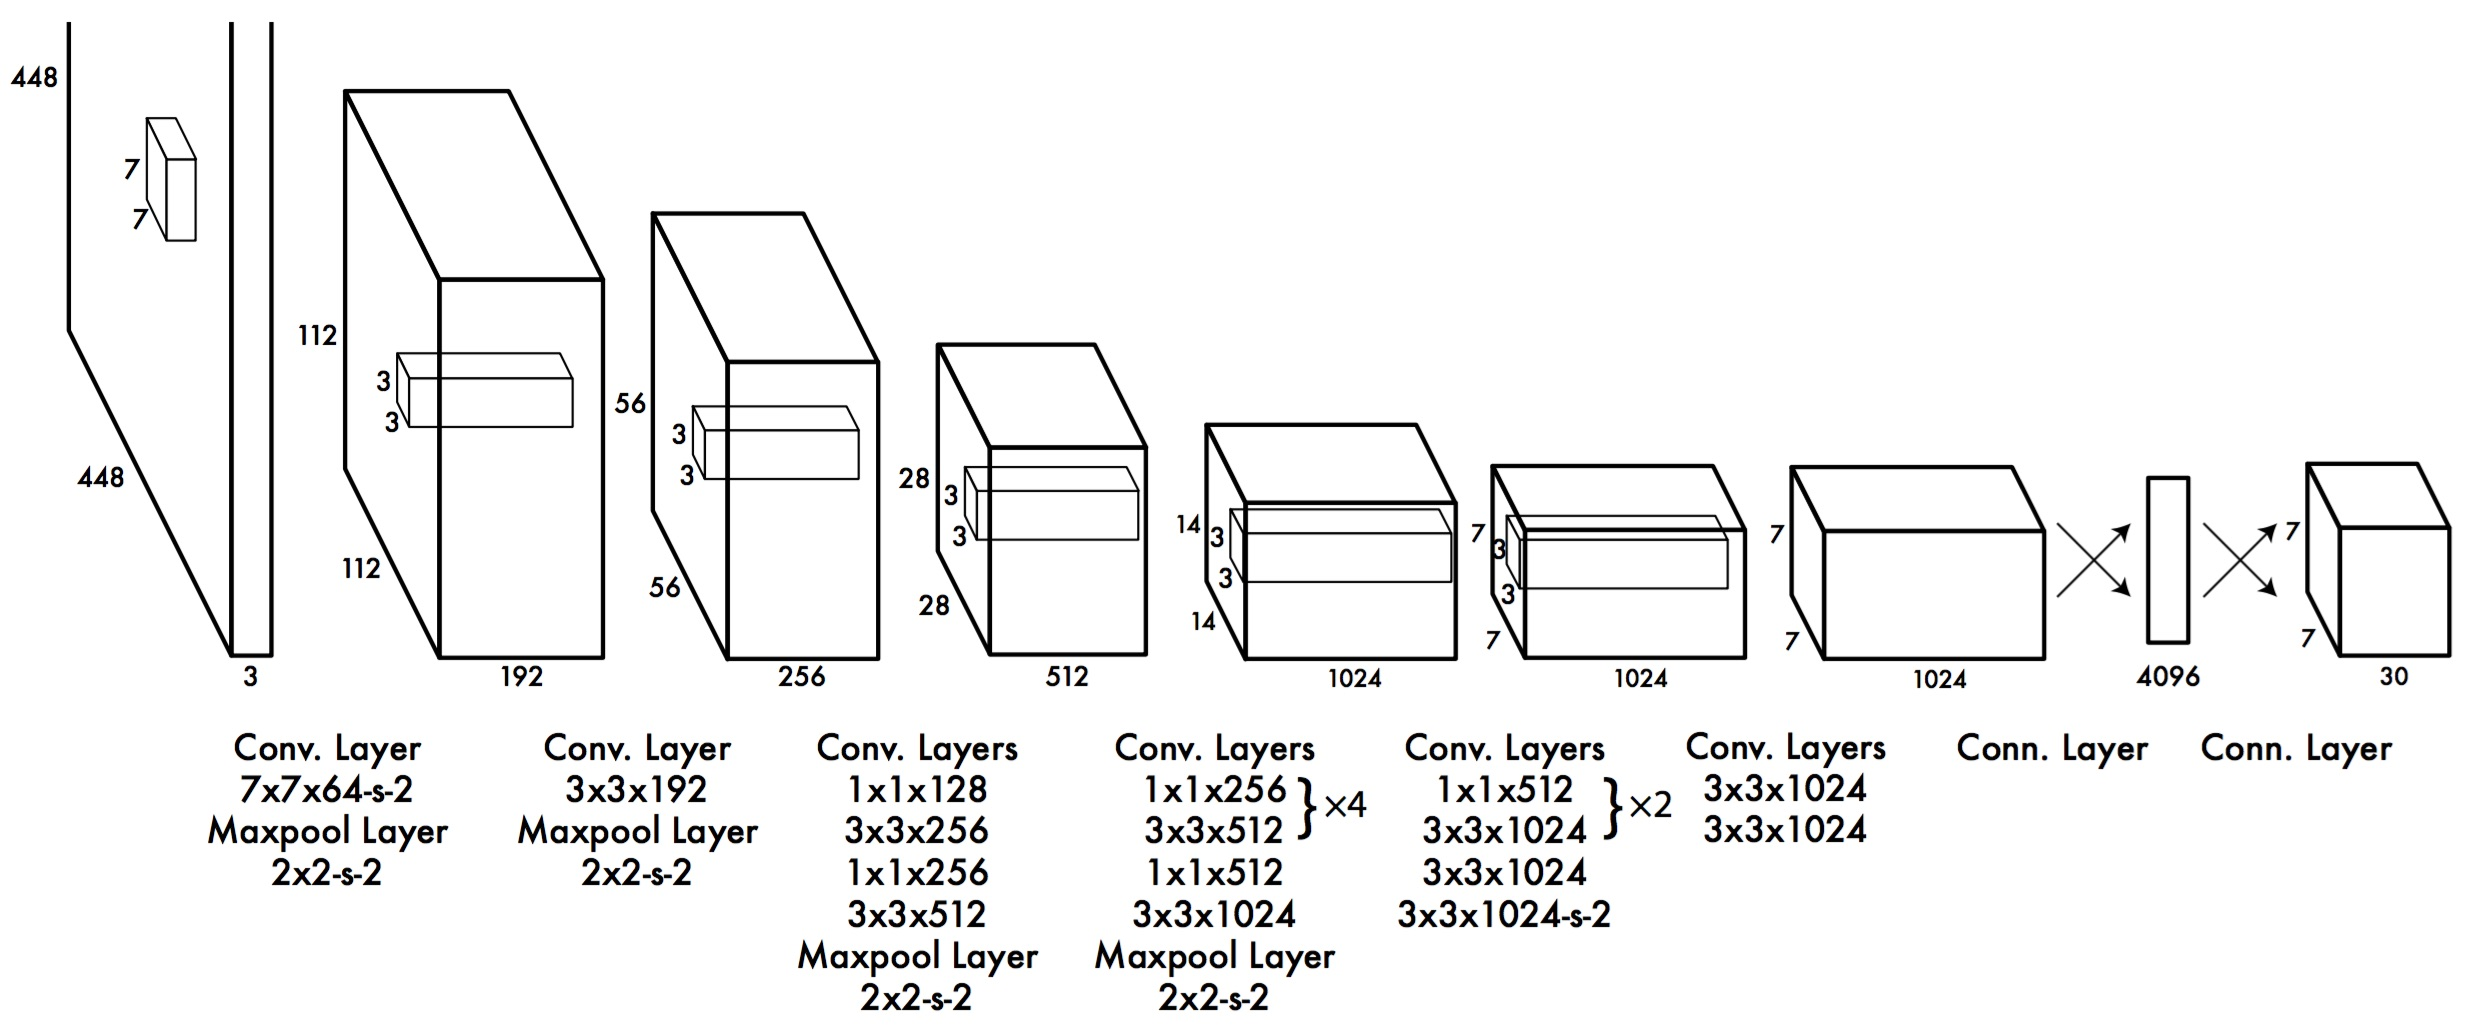
\includegraphics[width=12cm,height=10cm,keepaspectratio]{figures/yolo_net.jpg}
\caption{YOLO neural network structure}
\label{yolo_net}
\end{figure}

\vspace{10mm}
\section{ System Architecture Overview}

As it has been mentioned earlier, the system proposed in this thesis is built on top of the YOLO Architecture using our  TensorFlow implemented port  which will help in making our training more efficient and faster. We must note that YOLO is designed to process images in sequence. Therefore, it has no concept of temporal or spatial continuity between sequential frames in a video. For instance, while video frames may be fed into YOLO sequentially, YOLO cannot determine which object detected in one frame corresponds to the same object in the next frame.  Our task is to re-implement, train, and test  YOLO using TensorFlow and TLD(Tracking-Learning-Detection) so that it can track objects within a video in real-time and build  an application for a UAV/drone that uses a open source SDK to integrate our computer vision algorithm in ground station and the UAV to identify and track objects transmitted on a live video feed.

Figure \ref{our_app_2} shows a diagram on how we implement YOLO in TensorFlow to detect objects in video files, pictures, and live video feeds:

\begin{figure}[h]
\setlength{\belowcaptionskip}{-30pt}
\centering
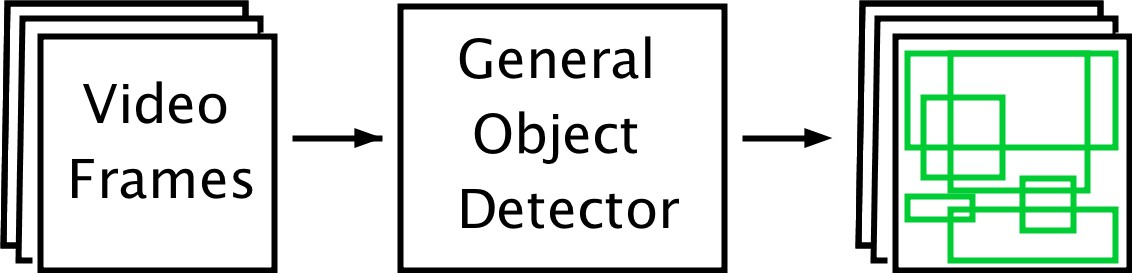
\includegraphics[scale=0.3]{figures/our_app_2.png}
\caption{YOLO in TensorFlow implementation diagram}
\label{our_app_2}
\end{figure}

\vspace{10mm}

Figure \ref{our_architecture} shows an overview on how our system is implemented. First, a video sequence is given as an input,  in our case, we will use a live video feed from a drone's camera.

\begin{figure}[h]
\setlength{\belowcaptionskip}{-10pt}
\centering
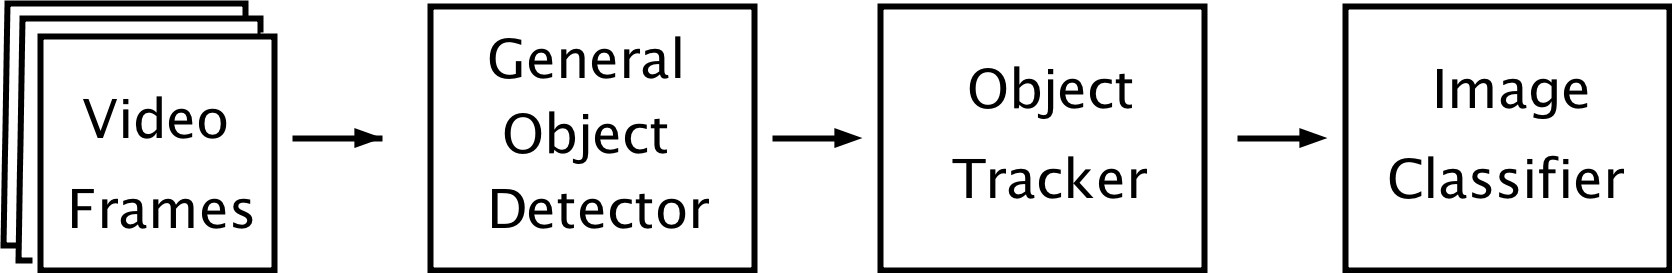
\includegraphics[scale=0.3]{figures/our_app.png}
\caption{Block Diagram of the system architechture}
\label{our_architecture}
\end{figure}

\vspace{200mm}

The code snippet below shows how we access live video feed from a drone's camera and download it to our mobile device:

\vspace{5mm}
\begin{lstlisting}
// videofeed.py
import cv2
import numpy as np
import dronekit

// Create a VideoCapture object
cap = cv2.VideoCapture('./sololink.sdp')
// Check if camera opened successfully
if (cap.isOpened() == False): 
  print("Unable to read camera feed")
// Default resolutions of the frame are obtained.The default resolutions are system dependent.
// We convert the resolutions from float to integer.
frame_width = int(cap.get(3))
frame_height = int(cap.get(4))
// Define the codec and create VideoWriter object.The output is stored in 'outpy.avi' file.
out = cv2.VideoWriter('outpy.avi',cv2.VideoWriter_fourcc('M','J','P','G'), 10, (frame_width,frame_height))
while(True):
  ret, frame = cap.read()
  if ret == True: 
    // Write the frame into the file 'output.avi'
    out.write(frame)
    // Display the resulting frame    
    cv2.imshow('frame',frame)
    // Press Q on keyboard to stop recording
    if cv2.waitKey(1) & 0xFF == ord('q'):
      break
  // Break the loop
  else:
    break 
// When everything done, release the video capture and video write objects
cap.release()
out.release()
// Closes all the frames
cv2.destroyAllWindows() 
// videofeed.py
\end{lstlisting}

%\vspace{14mm}
\pagebreak
Detecting and classifying an object from the video feed or video sequence is done using our TensorFlow implementation of YOLO. The code snippet below shows how we proceed to implement our object detection algorithm.

\vspace{5mm}

\begin{lstlisting}
// detect.py
import os
import argparse
import configparser
import importlib
import itertools
from PIL import Image, ExifTags
import numpy as np
import matplotlib.pyplot as plt
import matplotlib.patches as patches
import tensorflow as tf
import tensorflow.contrib.slim as slim
import utils.preprocess
import utils.postprocess

def std(image):
    return utils.preprocess.per_image_standardization(image)

def darknet(image):
    return image / 255.

def read_image(path):
    image = Image.open(path)
    for key in ExifTags.TAGS.keys():
        if ExifTags.TAGS[key] == 'Orientation':
            break
    try:
        exif = dict(image._getexif().items())
    except AttributeError:
        return image
    if exif[key] == 3:
        image = image.rotate(180, expand=True)
    elif exif[key] == 6:
        image = image.rotate(270, expand=True)
    elif exif[key] == 8:
        image = image.rotate(90, expand=True)
    return image

def detect(sess, model, names, image, path):
    preprocess = eval(args.preprocess)
    _, height, width, _ = image.get_shape().as_list()
    _image = read_image(path)
    image_original = np.array(np.uint8(_image))
    if len(image_original.shape) == 2:
        image_original = np.repeat(np.expand_dims(image_original, -1), 3, 2)
    image_height, image_width, _ = image_original.shape
    image_std = preprocess(np.array(np.uint8(_image.resize((width, height)))).astype(np.float32))
    feed_dict = {image: np.expand_dims(image_std, 0)}
    tensors = [model.conf, model.xy_min, model.xy_max]
    conf, xy_min, xy_max = sess.run([tf.check_numerics(t, t.op.name) for t in tensors], feed_dict=feed_dict)
    boxes = utils.postprocess.non_max_suppress(conf[0], xy_min[0], xy_max[0], args.threshold, args.threshold_iou)
    scale = [image_width / model.cell_width, image_height / model.cell_height]
    fig = plt.figure()
    ax = fig.gca()
    ax.imshow(image_original)
    colors = [prop['color'] for _, prop in zip(names, itertools.cycle(plt.rcParams['axes.prop_cycle']))]
    cnt = 0
    for _conf, _xy_min, _xy_max in boxes:
        index = np.argmax(_conf)
        if _conf[index] > args.threshold:
            wh = _xy_max - _xy_min
            _xy_min = _xy_min * scale
            _wh = wh * scale
            linewidth = min(_conf[index] * 10, 3)
            ax.add_patch(patches.Rectangle(_xy_min, _wh[0], _wh[1], linewidth=linewidth, edgecolor=colors[index], facecolor='none'))
            ax.annotate(names[index] + ' (%.1f%%)' % (_conf[index] * 100), _xy_min, color=colors[index])
            cnt += 1
    fig.canvas.set_window_title('%d objects detected' % cnt)
    ax.set_xticks([])
    ax.set_yticks([])
    return fig

def main():
    model = config.get('config', 'model')
    yolo = importlib.import_module('model.' + model)
    width = config.getint(model, 'width')
    height = config.getint(model, 'height')
    with tf.Session() as sess:
        image = tf.placeholder(tf.float32, [1, height, width, 3], name='image')
        builder = yolo.Builder(args, config)
        builder(image)
        global_step = tf.contrib.framework.get_or_create_global_step()
        model_path = tf.train.latest_checkpoint(utils.get_logdir(config))
        tf.logging.info('load ' + model_path)
        slim.assign_from_checkpoint_fn(model_path, tf.global_variables())(sess)
        tf.logging.info('global_step=%d' % sess.run(global_step))
        path = os.path.expanduser(os.path.expandvars(args.path))
        if os.path.isfile(path):
            detect(sess, builder.model, builder.names, image, path)
            plt.show()
        else:
            for dirpath, _, filenames in os.walk(path):
                for filename in filenames:
                    if os.path.splitext(filename)[-1].lower() in args.exts:
                        _path = os.path.join(dirpath, filename)
                        print(_path)
                        detect(sess, builder.model, builder.names, image, _path)
                        plt.show()

def make_args():
    parser = argparse.ArgumentParser()
    parser.add_argument('path', help='input image path')
    parser.add_argument('-c', '--config', nargs='+', default=['config.ini'], help='config file')
    parser.add_argument('-p', '--preprocess', default='std', help='the preprocess function')
    parser.add_argument('-t', '--threshold', type=float, default=0.3)
    parser.add_argument('--threshold_iou', type=float, default=0.4, help='IoU threshold')
    parser.add_argument('-e', '--exts', nargs='+', default=['.jpg', '.png'])
    parser.add_argument('--level', default='info', help='logging level')
    return parser.parse_args()

if __name__ == '__main__':
    args = make_args()
    config = configparser.ConfigParser()
    utils.load_config(config, args.config)
    if args.level:
        tf.logging.set_verbosity(args.level.upper())
    main()
// detect.py
\end{lstlisting}

\vspace{5mm}
Using OpenCV feature extraction algorithm, we track a set of features across the video sequence. Once the features have been detected in the object throughout the video frames, it will identify the same points accross the live video feed. To track the detected object over time,  we use TLD (Tracking-Detection-Learning) algorithm to learn the objects appearance and detect it whenever it moves or appears in the video feed.

\vspace{5mm}

\begin{lstlisting}
//tracker.py
//Tracking using TLD in OpenCV
import numpy as np
import cv2
import sys

if len(sys.argv) != 2:
    print('Input video name is missing')
    exit()

print('Select 3 tracking targets')

cv2.namedWindow("tracking")
camera = cv2.VideoCapture(sys.argv[1])
tracker = cv2.MultiTracker_create()
init_once = False

ok, image=camera.read()
if not ok:
    print('Failed to read video')
    exit()

bbox1 = cv2.selectROI('tracking', image)
bbox2 = cv2.selectROI('tracking', image)
bbox3 = cv2.selectROI('tracking', image)

while camera.isOpened():
    ok, image=camera.read()
    if not ok:
        print 'no image to read'
        break

    if not init_once:
        ok = tracker.add(cv2.TrackerMIL_create(), image, bbox1)
        ok = tracker.add(cv2.TrackerMIL_create(), image, bbox2)
        ok = tracker.add(cv2.TrackerMIL_create(), image, bbox3)
        init_once = True

    ok, boxes = tracker.update(image)
    print ok, boxes

    for newbox in boxes:
        p1 = (int(newbox[0]), int(newbox[1]))
        p2 = (int(newbox[0] + newbox[2]), int(newbox[1] + newbox[3]))
        cv2.rectangle(image, p1, p2, (200,0,0))

    cv2.imshow('tracking', image)
    k = cv2.waitKey(1)
    if k == 27 : break # esc presse
//tracker.py
\end{lstlisting}

\vspace{5mm}
\section{Training Our Network: Dataset}

Even though, our ultimate goal is to use a dataset that offers more advantages to our application in terms of training as well as testing such as COCO. Initially and for faster prototyping, we have used the PASCAL VOC dataset to train and test the functionality of our network. This training data consists of a set of images; each image has an annotation file giving a bounding box with coordinates and object class label for each object in one of  twenty classes present in the image.

The data has been split into 50\% for training/validation and 50\% for testing. The distributions of images and objects by class are approximately equal across the training/validation and test sets. In total there are 9,963 images, containing 24,640 annotated objects.

The CNN learns high-quality, hierarchical features automatically, eliminating the need for hand-selected features.

\vspace{5mm}
Below, a code snippet shows how we implement training for our network in figure \ref{retrained_model}:

\begin{lstlisting}
//train.py
import os
import argparse
import configparser
import importlib
import shutil
import time
import inspect
import multiprocessing
import tensorflow as tf
import tensorflow.contrib.slim as slim
import utils.data


def summary_scalar(config):
    try:
        reduce = eval(config.get('summary', 'scalar_reduce'))
        for t in utils.match_tensor(config.get('summary', 'scalar')):
            name = t.op.name
            if len(t.get_shape()) > 0:
                t = reduce(t)
                tf.logging.warn(name + ' is not a scalar tensor, reducing by ' + reduce.__name__)
            tf.summary.scalar(name, t)
    except (configparser.NoSectionError, configparser.NoOptionError):
        tf.logging.warn(inspect.stack()[0][3] + ' disabled')


def summary_image(config):
    try:
        for t in utils.match_tensor(config.get('summary', 'image')):
            name = t.op.name
            channels = t.get_shape()[-1].value
            if channels not in (1, 3, 4):
                t = tf.expand_dims(tf.reduce_sum(t, -1), -1)
            tf.summary.image(name, t, config.getint('summary', 'image_max'))
    except (configparser.NoSectionError, configparser.NoOptionError):
        tf.logging.warn(inspect.stack()[0][3] + ' disabled')


def summary_histogram(config):
    try:
        for t in utils.match_tensor(config.get('summary', 'histogram')):
            tf.summary.histogram(t.op.name, t)
    except (configparser.NoSectionError, configparser.NoOptionError):
        tf.logging.warn(inspect.stack()[0][3] + ' disabled')


def summary(config):
    summary_scalar(config)
    summary_image(config)
    summary_histogram(config)


def get_optimizer(config, name):
    section = 'optimizer_' + name
    return {
        'adam': lambda learning_rate: tf.train.AdamOptimizer(learning_rate, config.getfloat(section, 'beta1'), config.getfloat(section, 'beta2'), config.getfloat(section, 'epsilon')),
        'adadelta': lambda learning_rate: tf.train.AdadeltaOptimizer(learning_rate, config.getfloat(section, 'rho'), config.getfloat(section, 'epsilon')),
        'adagrad': lambda learning_rate: tf.train.AdagradOptimizer(learning_rate, config.getfloat(section, 'initial_accumulator_value')),
        'momentum': lambda learning_rate: tf.train.MomentumOptimizer(learning_rate, config.getfloat(section, 'momentum')),
        'rmsprop': lambda learning_rate: tf.train.RMSPropOptimizer(learning_rate, config.getfloat(section, 'decay'), config.getfloat(section, 'momentum'), config.getfloat(section, 'epsilon')),
        'ftrl': lambda learning_rate: tf.train.FtrlOptimizer(learning_rate, config.getfloat(section, 'learning_rate_power'), config.getfloat(section, 'initial_accumulator_value'), config.getfloat(section, 'l1_regularization_strength'), config.getfloat(section, 'l2_regularization_strength')),
        'gd': lambda learning_rate: tf.train.GradientDescentOptimizer(learning_rate),
    }[name]


def main():
    model = config.get('config', 'model')
    logdir = utils.get_logdir(config)
    if args.delete:
        tf.logging.warn('delete logging directory: ' + logdir)
        shutil.rmtree(logdir, ignore_errors=True)
    cachedir = utils.get_cachedir(config)
    with open(os.path.join(cachedir, 'names'), 'r') as f:
        names = [line.strip() for line in f]
    width = config.getint(model, 'width')
    height = config.getint(model, 'height')
    cell_width, cell_height = utils.calc_cell_width_height(config, width, height)
    tf.logging.warn('(width, height)=(%d, %d), (cell_width, cell_height)=(%d, %d)' % (width, height, cell_width, cell_height))
    yolo = importlib.import_module('model.' + model)
    paths = [os.path.join(cachedir, profile + '.tfrecord') for profile in args.profile]
    num_examples = sum(sum(1 for _ in tf.python_io.tf_record_iterator(path)) for path in paths)
    tf.logging.warn('num_examples=%d' % num_examples)
    with tf.name_scope('batch'):
        image_rgb, labels = utils.data.load_image_labels(paths, len(names), width, height, cell_width, cell_height, config)
        with tf.name_scope('per_image_standardization'):
            image_std = tf.image.per_image_standardization(image_rgb)
        batch = tf.train.shuffle_batch((image_std,) + labels, batch_size=args.batch_size,
            capacity=config.getint('queue', 'capacity'), min_after_dequeue=config.getint('queue', 'min_after_dequeue'),
            num_threads=multiprocessing.cpu_count()
        )
    global_step = tf.contrib.framework.get_or_create_global_step()
    builder = yolo.Builder(args, config)
    builder(batch[0], training=True)
    with tf.name_scope('total_loss') as name:
        builder.create_objectives(batch[1:])
        total_loss = tf.losses.get_total_loss(name=name)
    variables_to_restore = slim.get_variables_to_restore(exclude=args.exclude)
    with tf.name_scope('optimizer'):
        try:
            decay_steps = config.getint('exponential_decay', 'decay_steps')
            decay_rate = config.getfloat('exponential_decay', 'decay_rate')
            staircase = config.getboolean('exponential_decay', 'staircase')
            learning_rate = tf.train.exponential_decay(args.learning_rate, global_step, decay_steps, decay_rate, staircase=staircase)
            tf.logging.warn('using a learning rate start from %f with exponential decay (decay_steps=%d, decay_rate=%f, staircase=%d)' % (args.learning_rate, decay_steps, decay_rate, staircase))
        except (configparser.NoSectionError, configparser.NoOptionError):
            learning_rate = args.learning_rate
            tf.logging.warn('using a staionary learning rate %f' % args.learning_rate)
        optimizer = get_optimizer(config, args.optimizer)(learning_rate)
        tf.logging.warn('optimizer=' + args.optimizer)
        train_op = slim.learning.create_train_op(total_loss, optimizer, global_step,
            clip_gradient_norm=args.gradient_clip, summarize_gradients=config.getboolean('summary', 'gradients'),
        )
    if args.transfer:
        path = os.path.expanduser(os.path.expandvars(args.transfer))
        tf.logging.warn('transferring from ' + path)
        init_assign_op, init_feed_dict = slim.assign_from_checkpoint(path, variables_to_restore)
        def init_fn(sess):
            sess.run(init_assign_op, init_feed_dict)
            tf.logging.warn('transferring from global_step=%d, learning_rate=%f' % sess.run((global_step, learning_rate)))
    else:
        init_fn = lambda sess: tf.logging.warn('global_step=%d, learning_rate=%f' % sess.run((global_step, learning_rate)))
    summary(config)
    tf.logging.warn('tensorboard --logdir ' + logdir)
    slim.learning.train(train_op, logdir, master=args.master, is_chief=(args.task == 0),
        global_step=global_step, number_of_steps=args.steps, init_fn=init_fn,
        summary_writer=tf.summary.FileWriter(os.path.join(logdir, args.logname)),
        save_summaries_secs=args.summary_secs, save_interval_secs=args.save_secs
    )


def make_args():
    parser = argparse.ArgumentParser()
    parser.add_argument('-c', '--config', nargs='+', default=['config.ini'], help='config file')
    parser.add_argument('-t', '--transfer', help='transferring model from a .ckpt file')
    parser.add_argument('-e', '--exclude', nargs='+', help='exclude variables while transferring')
    parser.add_argument('-p', '--profile', nargs='+', default=['train', 'val'])
    parser.add_argument('-s', '--steps', type=int, default=None, help='max number of steps')
    parser.add_argument('-d', '--delete', action='store_true', help='delete logdir')
    parser.add_argument('-b', '--batch_size', default=8, type=int, help='batch size')
    parser.add_argument('-o', '--optimizer', default='adam')
    parser.add_argument('-n', '--logname', default=time.strftime('%Y-%m-%d_%H-%M-%S'), help='the name for TensorBoard')
    parser.add_argument('-g', '--gradient_clip', default=0, type=float, help='gradient clip')
    parser.add_argument('-lr', '--learning_rate', default=1e-6, type=float, help='learning rate')
    parser.add_argument('--seed', type=int, default=None)
    parser.add_argument('--summary_secs', default=30, type=int, help='seconds to save summaries')
    parser.add_argument('--save_secs', default=600, type=int, help='seconds to save model')
    parser.add_argument('--level', help='logging level')
    parser.add_argument('--master', default='', help='master address')
    parser.add_argument('--task', type=int, default=0, help='task ID')
    return parser.parse_args()

if __name__ == '__main__':
    args = make_args()
    config = configparser.ConfigParser()
    utils.load_config(config, args.config)
    if args.level:
        tf.logging.set_verbosity(args.level.upper())
    main()
//train.py
\end{lstlisting}

\vspace{5mm}
\begin{figure}[h]
\setlength{\belowcaptionskip}{-30pt}
\centering
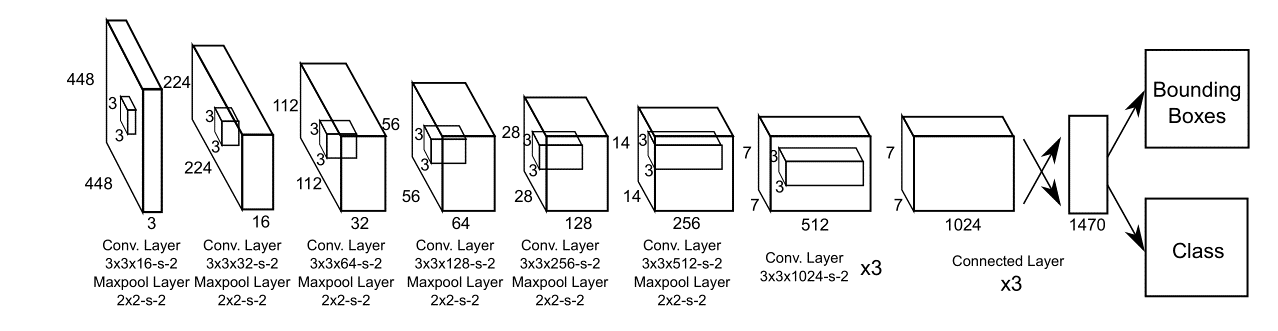
\includegraphics[scale=0.4]{figures/retrained_model.png}
\caption{Model trained  using PASCAL VOC with TensorFlow}
\label{retrained_model}
\end{figure}

\newpage
\section{Migrating Model to C++, JAVA, SWIFT, OBJECTIVE-C}

This is a tricky process to do since there is no official support for loading variables in C++ API. Google suggests assigning the trained weights as constants into the graph and save it down as a .pb (protobuf) file. However, this will double the necessary size of this file, which is very undesirable in, say, building mobile applications, for further information, refer to the official documentation forTensorflow C++ API  \url{https://www.tensorflow.org/api_docs/cc/}

To avoid this, one would have to build the graph all over again with all Variables replaced by Constants (we wouldn’t train any Deep Learning model on mobile device any time soon). Unfortunately, since there is no variable in this new graph, Tensorflow does not allow the convenient checkpointing, so one would need to resort to  \textbf{./binaries/.} while building this constant graph. In short, in order to produce a protobuf graph with optimal size for use in C++ , JAVA, and Objective-C++ API, one would need to use .weights files stored in \textbf{./binaries/.}

\vspace{5mm}
Below a snippet for exporting aour graph for use on mobile platforms:

\vspace{5mm}
\begin{lstlisting}
def savepb(self):
//Create a standalone const graph def
//So that C++ can load and run it.
//What's good abt it?
//1. Don't double the necessary size
//2. Convert on the fly - at any point you want
	
		darknet_ckpt = self.darknet
		flags_ckpt = self.FLAGS
		flags_ckpt.savepb = None //signal
		
		with self.graph.as_default() as g:
			for var in tf.trainable_variables():
				print var.name
				name = ':'.join(var.name.split(':')[:-1])
				var_name = name.split('-')
				val = var.eval(self.sess)
				l_idx = int(var_name[0])
				w_sig = var_name[-1]
				trained = var.eval(self.sess)
				darknet_ckpt.layers[l_idx].w[w_sig] = trained

		for layer in darknet_ckpt.layers:
			for ph in layer.h: //Set all placeholders to dfault val
				layer.h[ph] = self.feed[layer.h[ph]]['dfault']

		tfnet_ckpt = TFNet(darknet_ckpt, self.FLAGS)		
		tfnet_ckpt.sess = tf.Session(graph = tfnet_ckpt.graph)
		tfnet_ckpt.predict() //used for unit testing

		name = 'graph-{}.pb'.format(self.meta['model'])
		print 'Saving const graph def to {}'.format(name)
		graph_def = tfnet_ckpt.sess.graph_def
		tf.train.write_graph(graph_def,'./',name,False)
\end{lstlisting}


%\begin{figure}[h]
%\setlength{\belowcaptionskip}{-30pt}
%\centering
%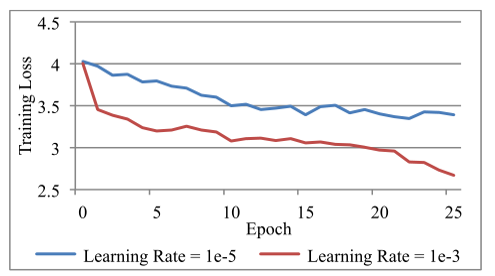
\includegraphics[scale=0.5]{figures/training_loss.png}
%\caption{Loss for various learning rates}
%\label{training_loss}
%\end{figure}
